\revise{}{
\subsection{Printing results}
In order to accurately manufacture adaptive width toolpaths using an off-the-shelf 3D printing system.
we need a model which relates the required width to process parameters such as movement speed and filament extrusion speed.
A different approach might be appropriate depending on whether the filament feeder is mounted directly on the print head (a.k.a. \emph{direct drive}) or the filament fed from the back of the printer to the print head via a \emph{Bowden tube}.
Because Bowden style 3D printing systems have the filament feeder relatively far away from the nozzle changing the internal pressure in the system requires a large amount of filament movement, which requires a prohibitive amount of time.

\paragraph{Back pressure compensation}
We therefore keep the internal pressure constant, and vary the movement speed instead.
%In order to accurately realize a varying bead width we vary the movement speed, while keeping the internal pressure in the system constant.
One approach would be keep the filament inflow $f$ (in \si{\milli\meter\cubed\per\second}) constant by varying movement speed accordingly \cite{Kuipers2018}.
However, that doesn't result in the intended filament outflow variation - see \cref{zero_back_pressure}.
We conjecture that the filament outflow is related to the total pressure in the system,
which depends not only on the amount of filament in between the feeder wheel and the nozzle (which we keep constant), 
but also depends on the back pressure that the previous layer exerts on the filament protruding from the nozzle.
We conjecture that the amount of back pressure is monotonically related to the requested line width and compensate for the back pressure using a simple linear model:

\begin{align}
 v(w) &= \frac{f(w)}{h w} \\ 
% f &\sim p \\
% p &= p_\text{in} + p_\text{ext} \\
% p_\text{in} &= C \\
% p_\text{ext} &\sim w \\
% p_\text{ext} &= w / w^* - 1 \\
% f &= f^* - k p_\text{ext} \\
 f(w) &= f_0 - k \left( w / w_0 - 1 \right) \\
 f_0 &= v_0 w_0 h 
% v &= \frac{f^* - k p_\text{ext}}{h w} \\ 
% v &= \frac{v^* w^* h - k (w / w^* - 1)}{h w}
\end{align}
where
$v(w)$ is the movement speed as a function of requested bead width $w$,
$f(w)$ is the filament outflow,
$f_0$ is a constant reference flow
and
$k$ is the amount of back pressure compensation.
Using increments of $0.1$ we established that using a factor of $k=1.1$ yields satisfactory bead width variation for our setup where
$v_0=\SI{30}{\milli\meter\per\second}$, 
$w_0=\SI{0.4}{\milli\meter}$.
See \cref{back_pressure}.
%
Test prints were performed on an unmodified Ultimaker S5 system,
with a standard  \SI{0.4}{\milli\meter} nozzle
and PLA filament
and a layer thickness of $h=\SI{0.1}{\milli\meter}$.
Because the machine instructions file format \emph{G-code} doesn't natively support adaptive width beads,
we discretize adaptive width extrusions into \SI{0.2}{\milli\meter} long segments of the average width.
The results can be viewed in \cref{prints}.


\begin{figure}
\centering
\setlength{\figwidth}{0.32\columnwidth}
\setlength{\figheight}{0.5\columnwidth}
\begin{subfigure}[t]{\figwidth}\centering
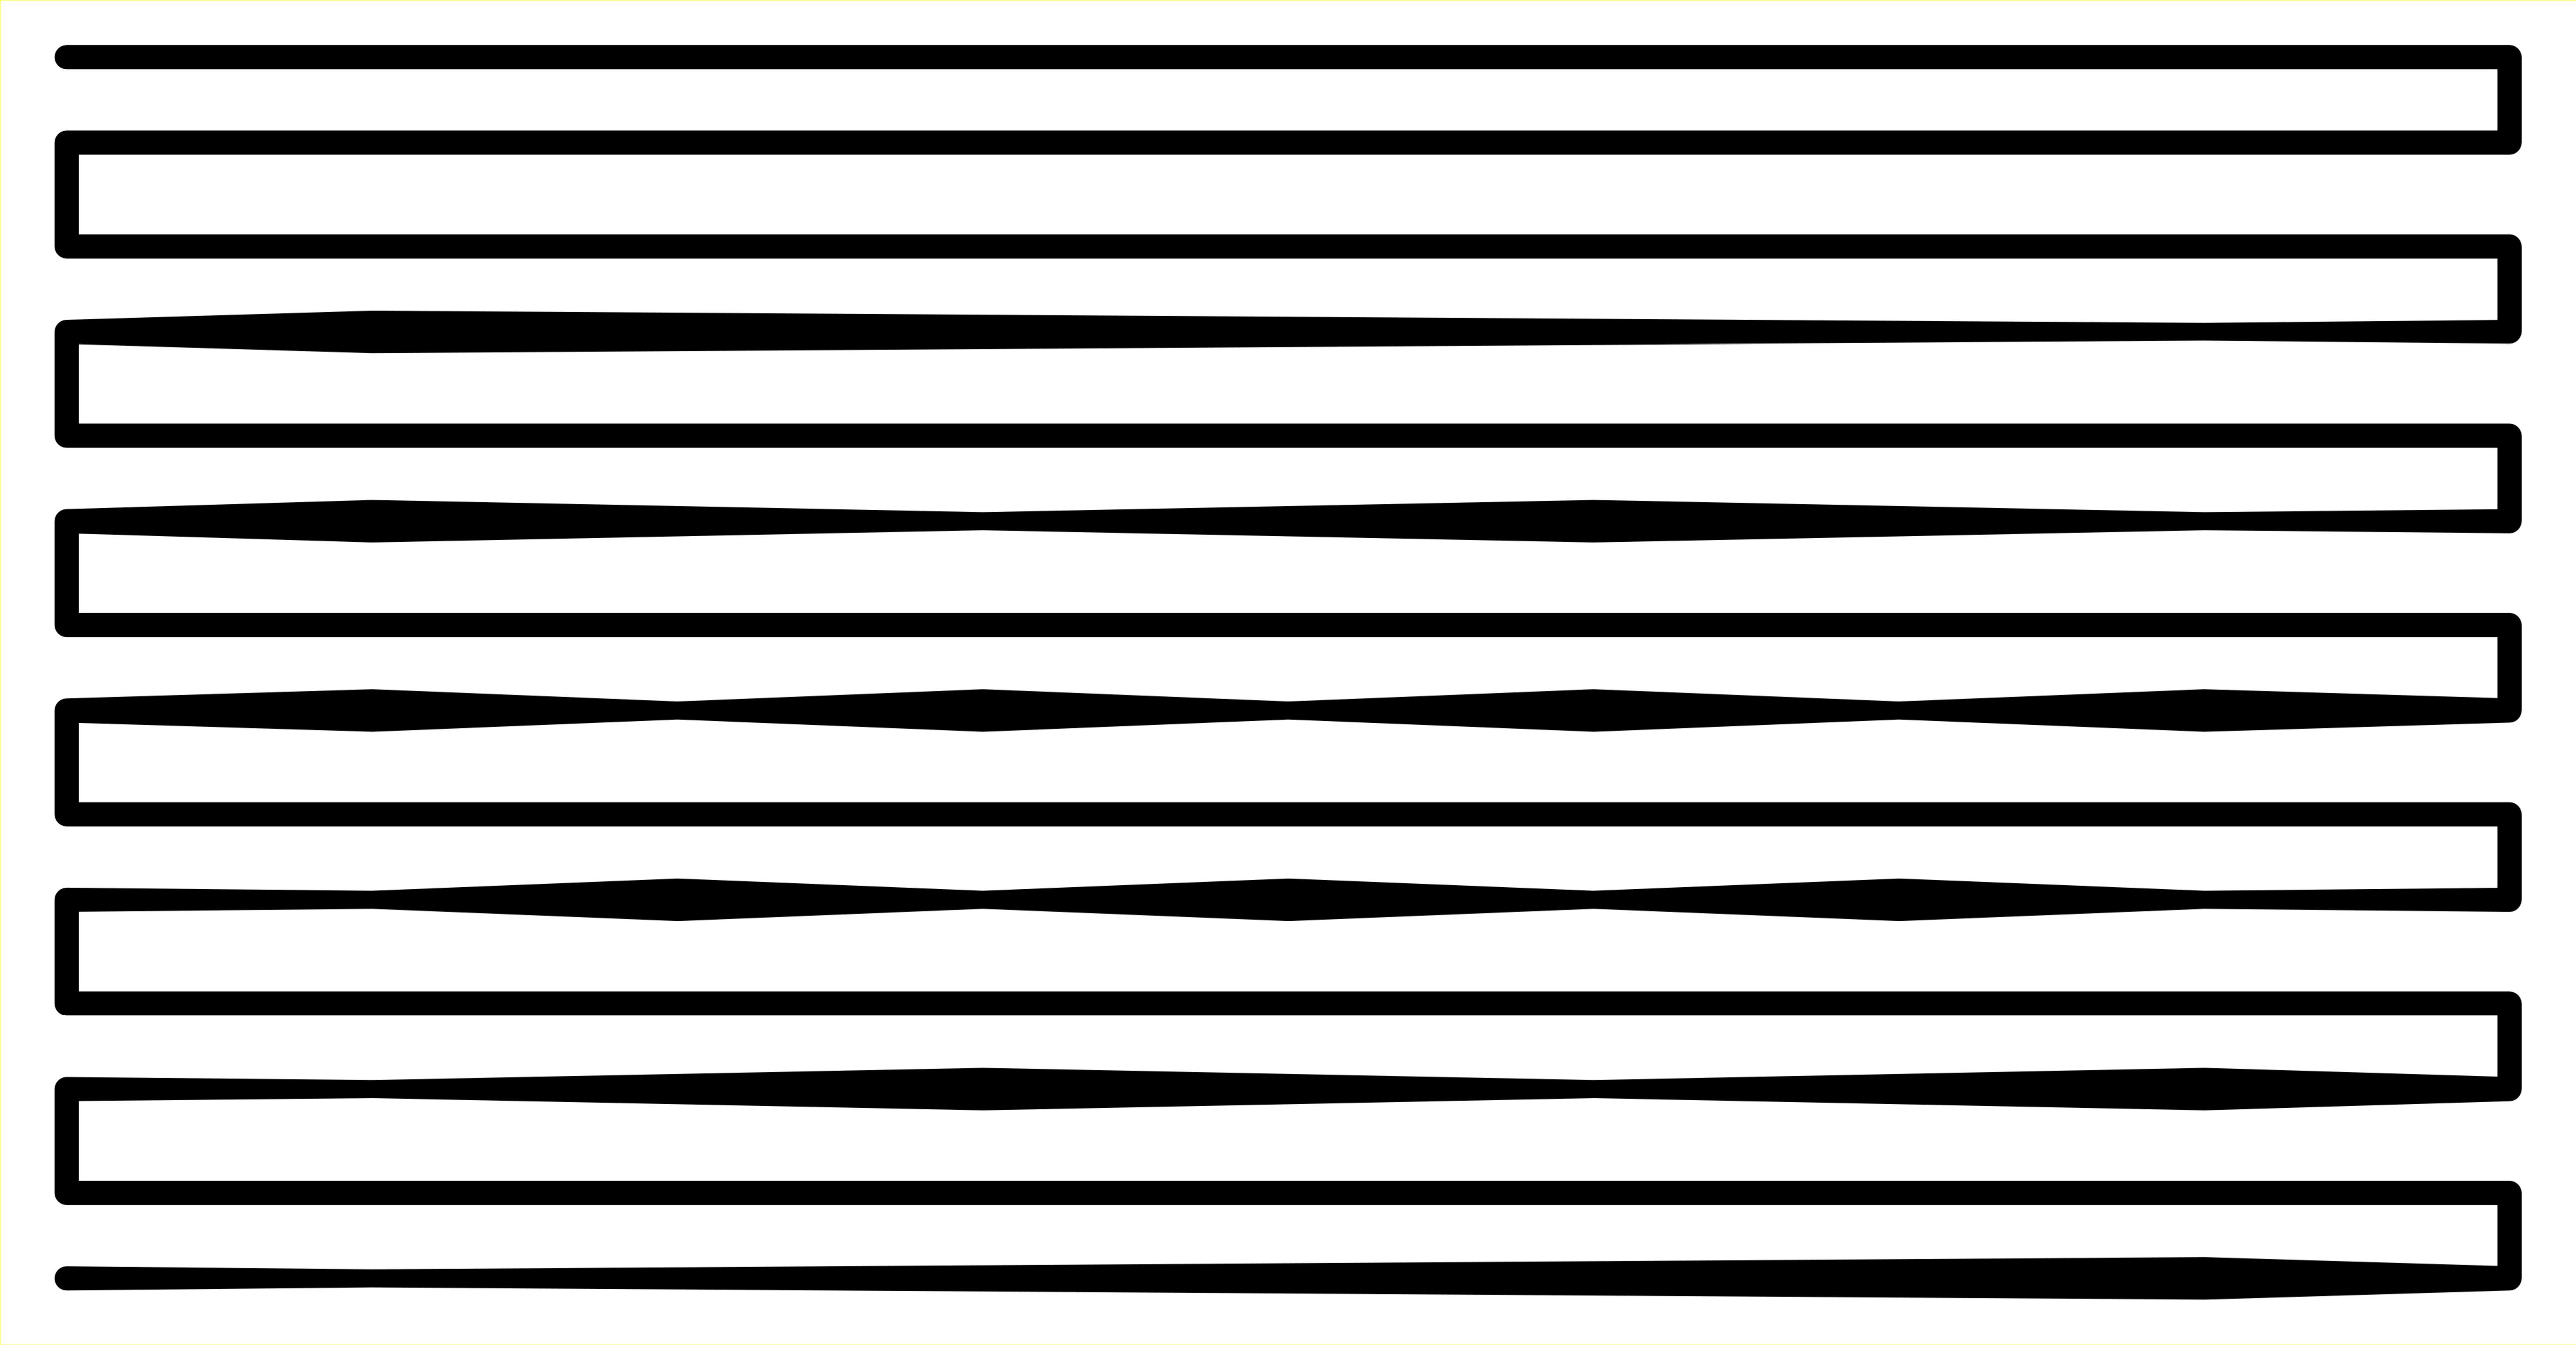
\includegraphics[angle=90,height=\figheight]{sources-validation-backpressure-compensation-target.pdf}
\caption{Target widths}\label{back_pressure_target}
\end{subfigure}
\begin{subfigure}[t]{\figwidth}\centering
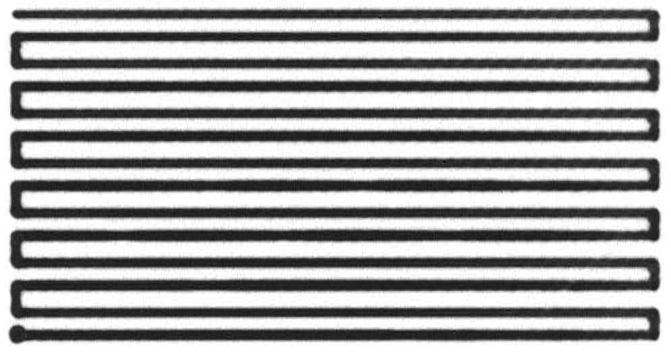
\includegraphics[angle=90,height=\figheight]{sources-validation-zero-backpressure-compensation.png}
\caption{Constant filament inflow (\si{\milli\meter\cubed\per\second})}\label{zero_back_pressure}
\end{subfigure}
\begin{subfigure}[t]{\figwidth}\centering
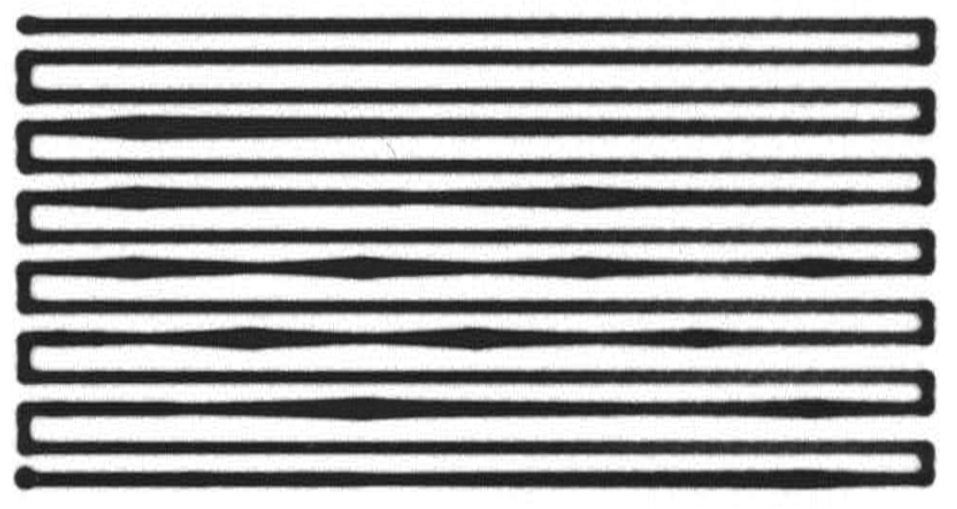
\includegraphics[angle=90,height=\figheight]{sources-validation-backpressure-compensation.png}
\caption{Back pressure compensation}\label{back_pressure}
\end{subfigure}
\caption{
Print results of varying width test on top of a dense white raft.
Trying to reproduce \subref{back_pressure_target} without back pressure compensation ($k=0$) yields worse results \subref{zero_back_pressure} than with back pressure compensation $k=1.1$ \subref{back_pressure}.
}
\label{back_pressure_compensation}
\end{figure}

% discussion of print results
\todo{TODO: discuss printed results.}

% adapted from 5.5 Discussion on implications
% limitations of back pressure compensation
Our back pressure compensation method effectively changes the speed to realize adaptive width,
but this approach is limited, since the movement speed is constrained by acceleration considerations near bends in the toolpath~\cite{Ertay2018}.
Moreover, as the layer height is decreased the back pressure becomes larger compared to the internal pressure, which might cause the back pressure compensation method to demand prohibitively slow movement speeds.
%
% direct drive & pressure advance
Accurate flow control can be further enhanced by using a direct drive hardware system and by employing \emph{pressure advance algorithms} which dynamically change the internal pressure \cite{tronvoll2019investigating}.
Conversely such a setup might benefit from some form of back pressure compensation as well.


\begin{figure}
\centering
\setlength{\figwidth}{0.9\columnwidth}
\begin{subfigure}{\figwidth}\centering
%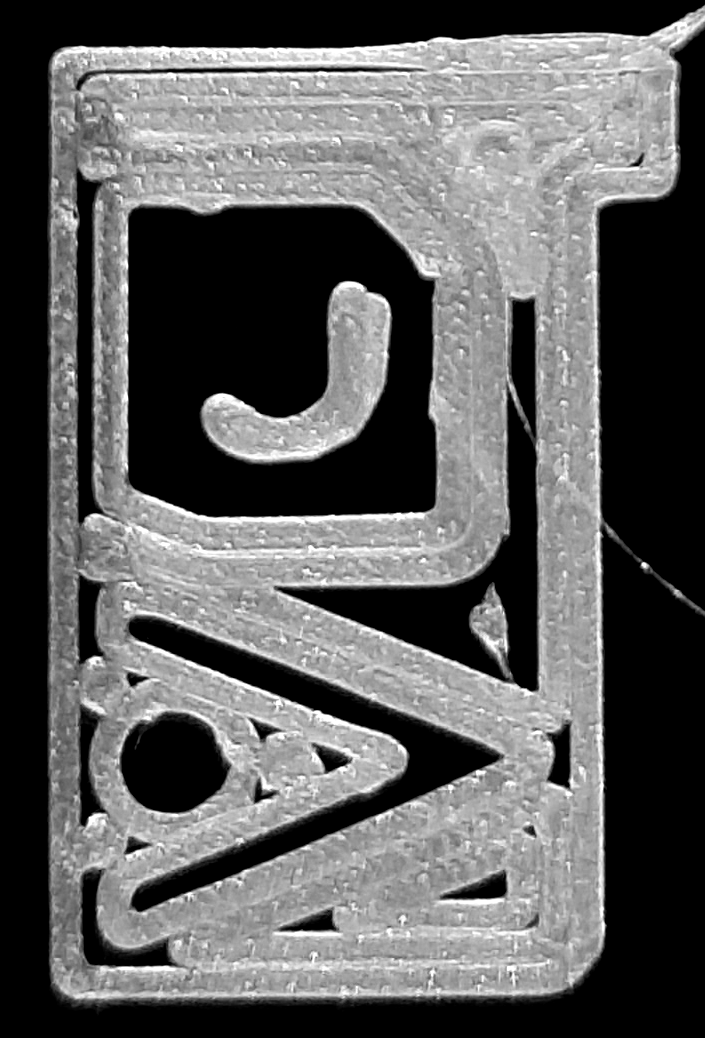
\includegraphics[height=\figheightTwo]{sources-applications-gMAT-naive.png}
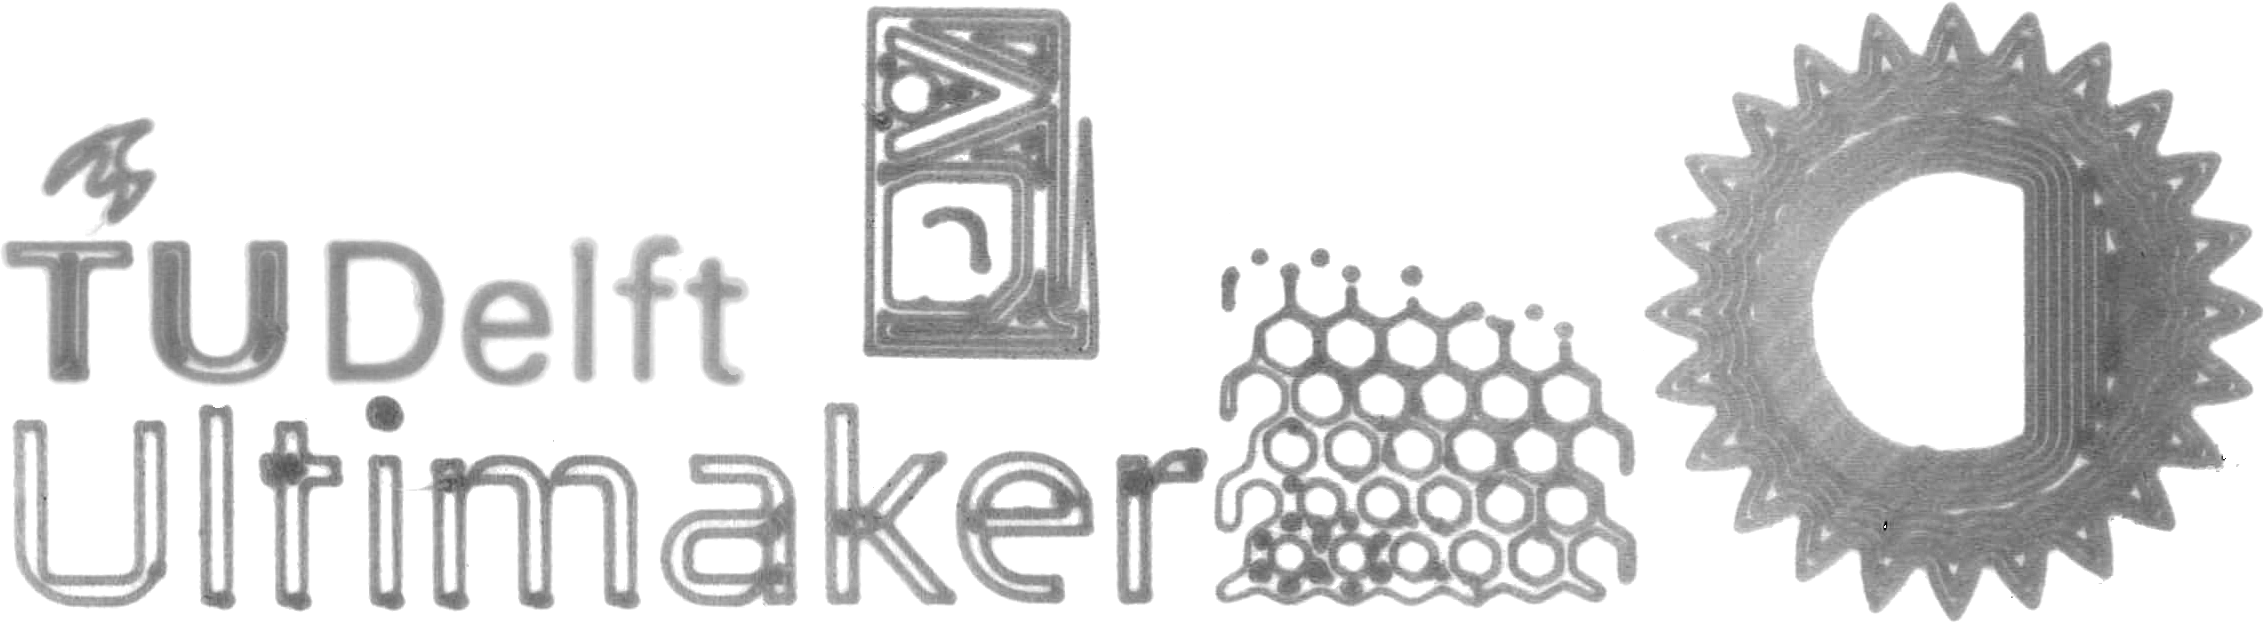
\includegraphics[width=\figwidth]{sources-applications-result-prints-naive-bw.png}
\caption{Uniform}\label{print_naive}
\end{subfigure}
\begin{subfigure}{\figwidth}\centering
%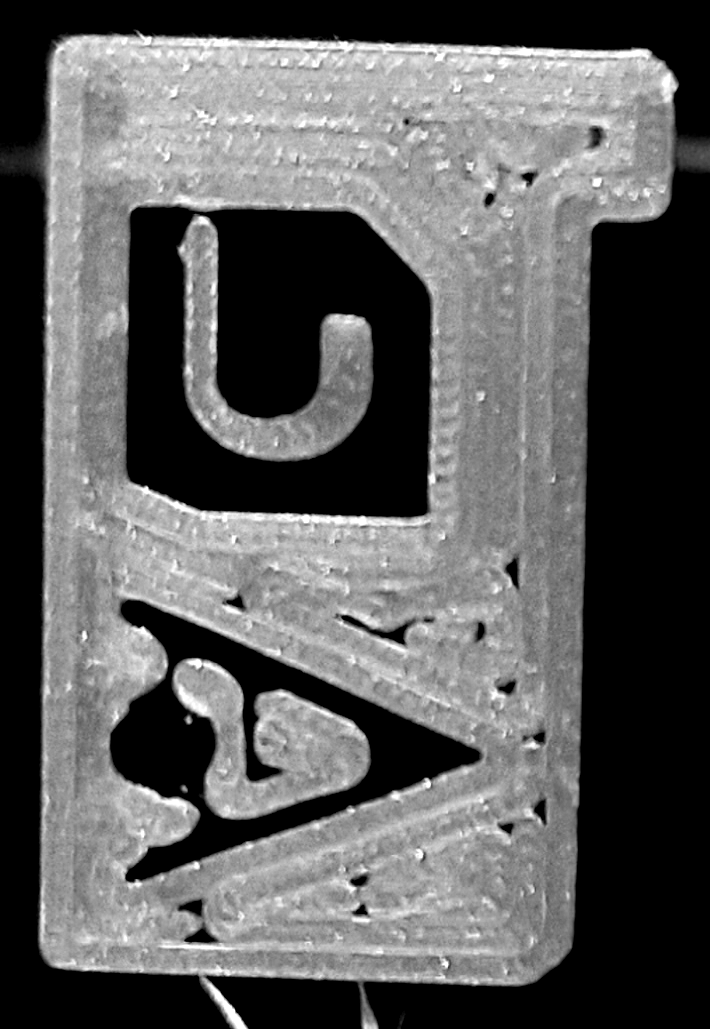
\includegraphics[height=\figheightTwo]{sources-applications-gMAT-center.png}
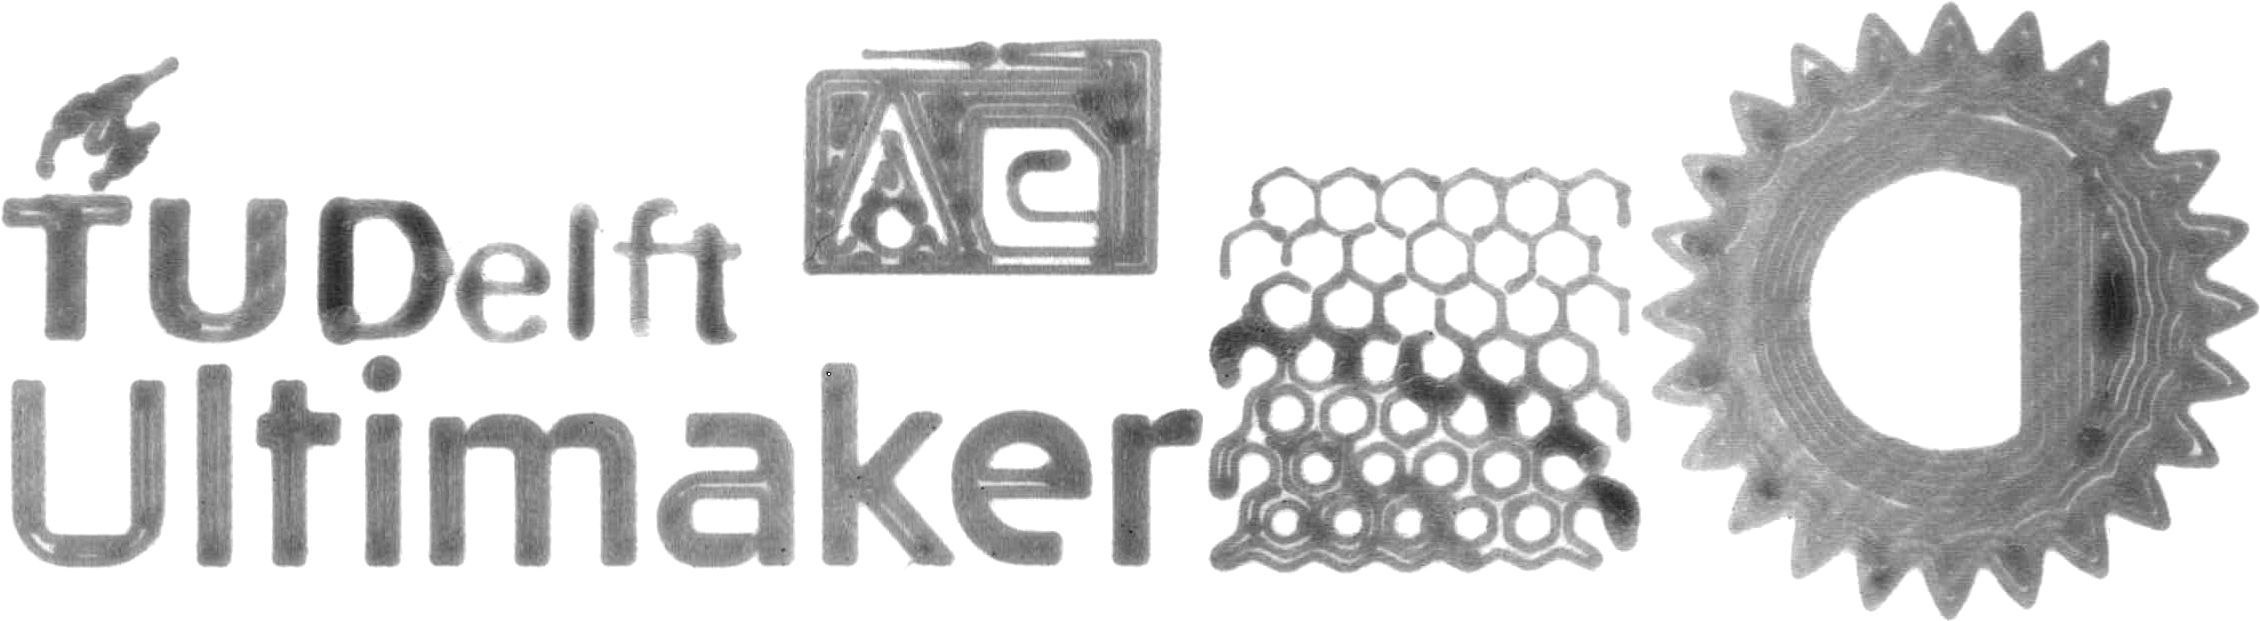
\includegraphics[width=\figwidth]{sources-applications-result-prints-center-bw.png}
\caption{Centered}\label{print_center}
\end{subfigure}
\begin{subfigure}{\figwidth}\centering
%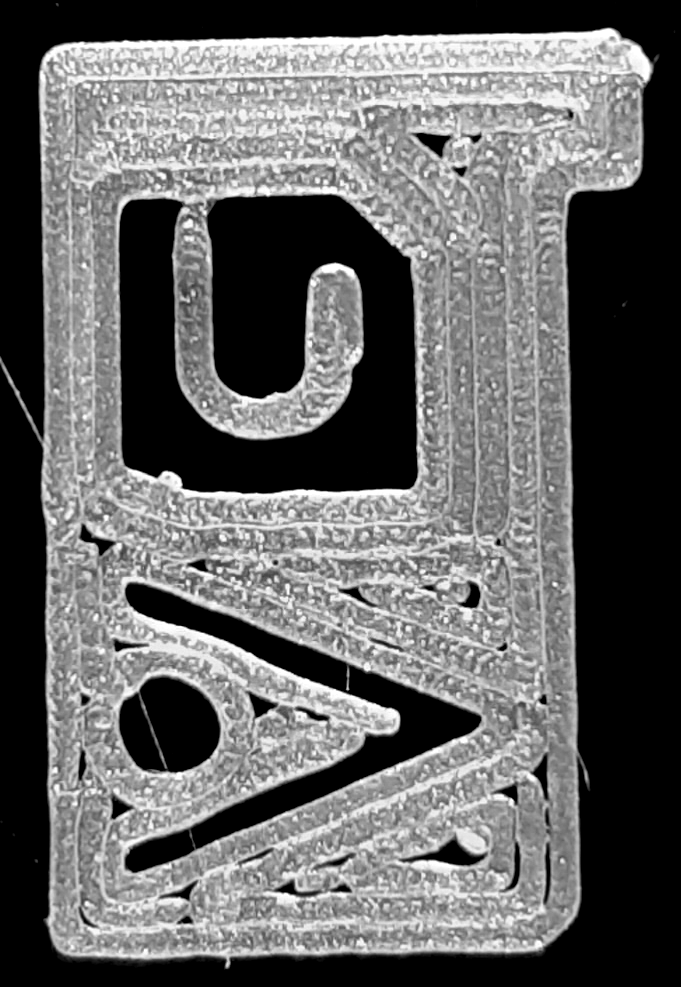
\includegraphics[height=\figheightTwo]{sources-applications-gMAT-inward.png}

\includegraphics[width=\figwidth]{sources-applications-result-prints-inward-bw.png}
\caption{Inward distributed}\label{print_inward}
\end{subfigure}
\caption{
Test shapes printed using the uniform scheme, centered scheme and the inward distributed scheme.
The uniform technique produces distinct underfill areas.
The centered scheme shows some defects due to inaccurate control of extreme deposition widths.
The inward distributed scheme produces the least defects.
}
\label{prints}
\end{figure}


}
